\chapter{Rappresentazione dei dati}
\label{sec:rappresentazione_dati}

In Fisica si ha spesso a che fare con enormi quantità di dati che non sono
facilmente interpretabili nella loro forma \emph{grezza}. Rappresentare
opportunamente tali dati ed estrarre l'informazione rilevante in una forma
intelligibile è uno dei compiti fondamentali del Fisico sperimentale.
In questo capitolo illustriamo brevemente alcune idee fondamentali
sull'argomento che svilupperemo ulteriormente nel seguito.


\section{Tabelle}

Supponiamo di voler stimare la velocità di un oggetto---vincolato a muoversi
su una retta---attraverso la misura della sua posizione ad intervalli di tempo
regolari. Per fissare le idee possiamo pensare di fotografare l'oggetto
ad istanti di tempo prefissati e di determinarne poi la posizione analizzando le
immagini così acquisite. Notiamo esplicitamente che, in questo schema, gli
errori sui tempi di misura sono \emph{trascurabili}, in un senso che avremo
modo di precisare in seguito, e quindi non rappresentati esplicitamente.
Detto $n$ il numero di fotogrammi, il nostro insieme di dati consiste in $n$
coppie ordinate di numeri (con i rispettivi errori), che possono essere
efficacemente rappresentate in forma tabellare come mostrato
nella tabella~\ref{tab:moto_uniforme_dati}.

\begin{table}[htbp]
  \tablehstack{
    \centering\begin{tabular}{ll}
      \hline
      Tempo~[s] & Posizione~[cm]\\
      \hline
      \hline
      $1.000$ & $20.5 \pm 2.5$ \\
$2.000$ & $28.7 \pm 2.5$ \\
$3.000$ & $35.4 \pm 2.5$ \\
$4.000$ & $43.1 \pm 2.5$ \\
$5.000$ & $51.8 \pm 2.5$ \\
$6.000$ & $54.6 \pm 2.5$ \\
$7.000$ & $64.1 \pm 2.5$ \\
$8.000$ & $69.7 \pm 2.5$ \\
$9.000$ & $77.5 \pm 2.5$
\\
      \hline
    \end{tabular}
  }{
    \caption{Esempio di rappresentazione di una serie di dati in forma tabellare.
      L'intestazione (cioè la prima riga) contiene un nome descrittivo per ogni
      colonna, con le rispettive unità di misura, di modo che la tabella risulti
      auto-contenuta. (In questo caso, visto che l'incertezza sulle posizioni
      è la stessa per tutte le righe, avremmo potuto riportarla una volta
      sola nell'intestazione oppure nella didascalia. Notiamo anche che
      nella colonna dei tempi non sono indicate esplicitamente le incertezze,
      ma gli zeri dopo la virgola sono significativi, il che indica che gli
      errori relativi sono dell'ordine dello $0.1\%$.)}
    \label{tab:moto_uniforme_dati}
  }
\end{table}

L'efficacia della formattazione di una tabella dipende in modo cruciale dal
contenuto, ed è argomento difficile da discutere in astratto. \`E tuttavia
buona norma, in generale, dare nomi il più possibile descrittivi alle colonne
ed indicare sempre le unità di misura, di modo che la tabella sia per quanto
possibile auto-esplicativa, ed il suo contenuto possa essere compreso senza
la necessità di informazioni esterne. (Da un punto di vista tipografico
sconsigliamo vivamente l'utilizzo di linee verticali nella composizione delle
tabelle.)


\section{Grafici di dispersione}

Un \emph{grafico di dispersione}%
\footnote{Per la verità il nome italiano, traduzione letterale dell'inglese
  \foreign{scatter plot}, non è molto usato, ma si trova talvolta in
  letteratura, per cui lo usiamo anche noi nello spirito di evitare il più
  possibile anglicismi.}%
---o \emph{grafico $xy$}, o semplicemente \emph{grafico}---è un diagramma in
cui coppie ordinate di dati (ad esempio misure dirette) sono visualizzate come
punti, eventualmente con le rispettive barre d'errore, su un piano cartesiano.
Si tratta di una delle più semplici rappresentazioni possibili di una serie
di dati---eppure è spesso utile, in pratica, per mettere in evidenza
proprietà rilevanti dei dati stessi che non sono immediatamente riconoscibili
nella rappresentazione in forma tabellare.

\pgffigone{moto_uniforme_dati}{
  Esempio di rappresentazione attraverso un grafico di dispersione dei dati
  contenuti nella tabella~\ref{tab:moto_uniforme_dati}. Si notino: la
  suddivisione regolare degli assi cartesiani, le etichette di testo che
  identificano le variabili rappresentate e le loro unità di misura, e le
  barre di errore---ove rappresentabili.
  Non c'è bisogno di sottolineare esplicitamente come la relazione lineare
  tra la variabile dipendente e quella indipendente sia immediatamente
  evidente nel grafico (cosa che non si può dire per la tabella).
}

Il grafico mostrato in figura~\ref{fig:moto_uniforme_dati} corrisponde ai dati
nella tabella~\ref{tab:moto_uniforme_dati}, ed ha tutte le caratteristiche
di base di un grafico realizzato correttamente:
\begin{itemize}
\item gli assi cartesiani sono suddivisi ad intervalli regolari in modo che
  le coordinate dei punti possano essere lette agevolmente;
\item le grandezze rappresentate in ascissa ed ordinata sono
  chiaramente identificate con una etichetta di testo e le rispettive unità di
  misura (tra parentesi quadre);
\item i dati sono rappresentati come punti e le barre di errore (in questo caso
  solo sulle ordinate) indicano graficamente l'intervallo di incertezza della
  misura.
\end{itemize}

Il frammento~\ref{snip:scatter_plot} illustra un programma \python\ minimale
per realizzare un grafico di dispersione simile a quello mostrato in
figura~\ref{fig:moto_uniforme_dati}. Si tratta di un esempio molto semplice,
ma vale la pena studiarlo in dettaglio, perché con semplici variazioni sul
tema vi permetterà nel seguito di realizzare una frazione significativa
dei grafici di cui avrete bisogno. Studiatelo riga per riga aiutandovi con
la documentazione di \matplotlib~\cite{matplotlibdoc} ed assicuratevi di aver
capito il significato di ogni singolo comando prima di procedere oltre.

\begin{snippet}[htb!]
  \bigskip % This is ugly and should be taken care of automagically.
  \hstack[0.625]{\begin{Verbatim}[label=\makebox{\href{https://github.com/unipi-physics-labs/lab1-notes/tree/main/snippy/scatter_plot.py}{https://github.com/.../scatter\_plot.py}},commandchars=\\\{\}]
\PY{k+kn}{import}\PY{+w}{ }\PY{n+nn}{numpy}\PY{+w}{ }\PY{k}{as}\PY{+w}{ }\PY{n+nn}{np}
\PY{k+kn}{from}\PY{+w}{ }\PY{n+nn}{matplotlib}\PY{+w}{ }\PY{k+kn}{import} \PY{n}{pyplot} \PY{k}{as} \PY{n}{plt}

\PY{c+c1}{\PYZsh{} Set matplotlib in interactive mode, so that plots are}
\PY{c+c1}{\PYZsh{} displayed on the screen as they are created.}
\PY{n}{plt}\PY{o}{.}\PY{n}{ion}\PY{p}{(}\PY{p}{)}

\PY{c+c1}{\PYZsh{} Definition of the data points.}
\PY{n}{t} \PY{o}{=} \PY{p}{[}\PY{l+m+mf}{1.0}\PY{p}{,} \PY{l+m+mf}{2.0}\PY{p}{,} \PY{l+m+mf}{3.0}\PY{p}{,} \PY{l+m+mf}{4.0}\PY{p}{,} \PY{l+m+mf}{5.0}\PY{p}{,} \PY{l+m+mf}{6.0}\PY{p}{,} \PY{l+m+mf}{7.0}\PY{p}{,} \PY{l+m+mf}{8.0}\PY{p}{,} \PY{l+m+mf}{9.0}\PY{p}{]}
\PY{n}{s} \PY{o}{=} \PY{p}{[}\PY{l+m+mf}{20.5}\PY{p}{,} \PY{l+m+mf}{28.7}\PY{p}{,} \PY{l+m+mf}{35.4}\PY{p}{,} \PY{l+m+mf}{43.1}\PY{p}{,} \PY{l+m+mf}{51.8}\PY{p}{,} \PY{l+m+mf}{54.6}\PY{p}{,} \PY{l+m+mf}{64.1}\PY{p}{,} \PY{l+m+mf}{69.7}\PY{p}{,} \PY{l+m+mf}{77.5}\PY{p}{]}
\PY{n}{sigma\PYZus{}s} \PY{o}{=} \PY{p}{[}\PY{l+m+mf}{2.5}\PY{p}{,} \PY{l+m+mf}{2.5}\PY{p}{,} \PY{l+m+mf}{2.5}\PY{p}{,} \PY{l+m+mf}{2.5}\PY{p}{,} \PY{l+m+mf}{2.5}\PY{p}{,} \PY{l+m+mf}{2.5}\PY{p}{,} \PY{l+m+mf}{2.5}\PY{p}{,} \PY{l+m+mf}{2.5}\PY{p}{,} \PY{l+m+mf}{2.5}\PY{p}{]}
\PY{c+c1}{\PYZsh{} Make the actual plot.}
\PY{n}{plt}\PY{o}{.}\PY{n}{errorbar}\PY{p}{(}\PY{n}{t}\PY{p}{,} \PY{n}{s}\PY{p}{,} \PY{n}{sigma\PYZus{}s}\PY{p}{,} \PY{n}{fmt}\PY{o}{=}\PY{l+s+s1}{\PYZsq{}}\PY{l+s+s1}{o}\PY{l+s+s1}{\PYZsq{}}\PY{p}{)}
\PY{c+c1}{\PYZsh{} Setup the axes labels.}
\PY{n}{plt}\PY{o}{.}\PY{n}{xlabel}\PY{p}{(}\PY{l+s+s1}{\PYZsq{}}\PY{l+s+s1}{Tempo [s]}\PY{l+s+s1}{\PYZsq{}}\PY{p}{)}
\PY{n}{plt}\PY{o}{.}\PY{n}{ylabel}\PY{p}{(}\PY{l+s+s1}{\PYZsq{}}\PY{l+s+s1}{Posizione [cm]}\PY{l+s+s1}{\PYZsq{}}\PY{p}{)}
\PY{c+c1}{\PYZsh{} Adjust the axis ranges (None means autoscale).}
\PY{n}{plt}\PY{o}{.}\PY{n}{axis}\PY{p}{(}\PY{p}{[}\PY{l+m+mf}{0.0}\PY{p}{,} \PY{l+m+mf}{10.0}\PY{p}{,} \PY{l+m+mf}{0.0}\PY{p}{,} \PY{k+kc}{None}\PY{p}{]}\PY{p}{)}
\end{Verbatim}
}{
    \caption{Esempio di programma in \python\ per generare, a partire dai dati
      in tabella~\ref{tab:moto_uniforme_dati}, un grafico di dispersione simile
      quello mostrato in figura~\ref{fig:moto_uniforme_dati}. I commenti
      dovrebbero essere d'aiuto per la comprensione.
      In questo caso i dati sono scritti direttamente all'interno del
      programma, ma nella vita reale---specialmente quando il numero di
      punti è alto---è più comune che essi siano letti da file.
    }
    \label{snip:scatter_plot}
  }
\end{snippet}


\section{Digressione: di nuovo su \python}

Prima di andare avanti abbiamo bisogno di soffermarci per un attimo su un paio
di argomenti per ampliare il nostro vocabolario di \python\ ed approfondire
alcuni aspetti specifici del suo ecosistema scientifico.


\subsection{Riutilizzo del codice: le funzioni}

Quando dobbiamo eseguire ripetutamente la stessa operazione è comodo includere
la sequenza di istruzioni elementari in una \emph{funzione} in modo da evitare
duplicazioni di codice e rendere il nostro programma più leggibile e
mantenibile. Abbiamo già visto esempi di funzioni nei
frammenti~\ref{snip:rounding} e \ref{snip:mean_stdev} e, come ogni linguaggio di
programmazione che si rispetti, \python\ permette all'utente di definire
funzioni addizionali arbitrarie.

\begin{snippet}[htb!]
  \bigskip % This is ugly and should be taken care of automagically.
  \hstack[0.56]{\begin{Verbatim}[label=\makebox{\href{https://github.com/unipi-physics-labs/statnotes/tree/main/snippy/func_def.py}{https://github.com/.../func\_def.py}},commandchars=\\\{\}]
\PY{k+kn}{import}\PY{+w}{ }\PY{n+nn}{numpy}\PY{+w}{ }\PY{k}{as}\PY{+w}{ }\PY{n+nn}{np}

\PY{k}{def}\PY{+w}{ }\PY{n+nf}{sum\PYZus{}err\PYZus{}prop}\PY{p}{(}\PY{n}{x}\PY{p}{,} \PY{n}{sigma\PYZus{}x}\PY{p}{,} \PY{n}{y}\PY{p}{,} \PY{n}{sigma\PYZus{}y}\PY{p}{)}\PY{p}{:}
\PY{+w}{    }\PY{l+s+sd}{\PYZdq{}\PYZdq{}\PYZdq{}Error propagation on the addition operation.}
\PY{l+s+sd}{    \PYZdq{}\PYZdq{}\PYZdq{}}
    \PY{n}{s\PYZus{}hat} \PY{o}{=} \PY{n}{x} \PY{o}{+} \PY{n}{y}
    \PY{n}{sigma\PYZus{}s} \PY{o}{=} \PY{n}{np}\PY{o}{.}\PY{n}{sqrt}\PY{p}{(}\PY{n}{sigma\PYZus{}x}\PY{o}{*}\PY{o}{*}\PY{l+m+mf}{2.0} \PY{o}{+} \PY{n}{sigma\PYZus{}y}\PY{o}{*}\PY{o}{*}\PY{l+m+mf}{2.0}\PY{p}{)}
    \PY{k}{return} \PY{n}{s\PYZus{}hat}\PY{p}{,} \PY{n}{sigma\PYZus{}s}

\PY{n}{s\PYZus{}hat}\PY{p}{,} \PY{n}{sigma\PYZus{}s} \PY{o}{=} \PY{n}{sum\PYZus{}err\PYZus{}prop}\PY{p}{(}\PY{l+m+mf}{1.0}\PY{p}{,} \PY{l+m+mf}{0.01}\PY{p}{,} \PY{l+m+mf}{2.0}\PY{p}{,} \PY{l+m+mf}{0.02}\PY{p}{)}
\PY{n+nb}{print}\PY{p}{(}\PY{l+s+sa}{f}\PY{l+s+s1}{\PYZsq{}}\PY{l+s+s1}{s = }\PY{l+s+si}{\PYZob{}}\PY{n}{s\PYZus{}hat}\PY{l+s+si}{:}\PY{l+s+s1}{.3f}\PY{l+s+si}{\PYZcb{}}\PY{l+s+s1}{ +/\PYZhy{} }\PY{l+s+si}{\PYZob{}}\PY{n}{sigma\PYZus{}s}\PY{l+s+si}{:}\PY{l+s+s1}{.3f}\PY{l+s+si}{\PYZcb{}}\PY{l+s+s1}{\PYZsq{}}\PY{p}{)}
\PY{n}{s\PYZus{}hat}\PY{p}{,} \PY{n}{sigma\PYZus{}s} \PY{o}{=} \PY{n}{sum\PYZus{}err\PYZus{}prop}\PY{p}{(}\PY{l+m+mf}{1.0}\PY{p}{,} \PY{l+m+mf}{0.01}\PY{p}{,} \PY{l+m+mf}{14.0}\PY{p}{,} \PY{l+m+mf}{0.2}\PY{p}{)}
\PY{n+nb}{print}\PY{p}{(}\PY{l+s+sa}{f}\PY{l+s+s1}{\PYZsq{}}\PY{l+s+s1}{s = }\PY{l+s+si}{\PYZob{}}\PY{n}{s\PYZus{}hat}\PY{l+s+si}{:}\PY{l+s+s1}{.2f}\PY{l+s+si}{\PYZcb{}}\PY{l+s+s1}{ +/\PYZhy{} }\PY{l+s+si}{\PYZob{}}\PY{n}{sigma\PYZus{}s}\PY{l+s+si}{:}\PY{l+s+s1}{.2f}\PY{l+s+si}{\PYZcb{}}\PY{l+s+s1}{\PYZsq{}}\PY{p}{)}

[Output]
s = 3.000 +/- 0.022
s = 15.00 +/- 0.20
\end{Verbatim}
}{
    \caption{Definizione di una funzione \python\ per la propagazione
      dell'errore statistico sulla somma $s = x + y$ di sue grandezze misurate
      con errori $\sigma_x$ e $\sigma_y$. La funzione accetta (nell'ordine)
      $x$, $\sigma_x$, $y$ e $\sigma_y$ come argomenti e restituisce
      (nell'ordine) $s$ e $\sigma_s$. Una volta definita, la funzione può
      essere richiamata più volte con valori arbitrari degli argomenti.
      Il testo incluso tra i due gruppi di tre virgolette serve a documentare
      brevemente l'utilizzo della funzione---non è strettamente necessario,
      ma è utile in generale.
    }
    \label{snip:func_def}
  }
\end{snippet}

Come illustrato nel frammento~\ref{snip:func_def}, una funzione può accettare
\emph{argomenti} (ossia variabili da utilizzare nel corpo della funzione stessa)
in ingresso, e può restituire valori in uscita. La sintassi per la
definizione delle funzioni in \python\ è estremamente più ricca di quanto
questo semplice esempio possa suggerire, ma per il momento quanto detto è
sufficiente ai nostri scopi.


\subsection{Lavorare con gli \nparray}

Il pacchetto \numpy\ è la libreria numerica alla base dell'intero
ecosistema scientifico di \python---ed il nucleo fondamentale di \numpy\
è costituito da un sistema estremamente potente e flessibile di \foreign{array}
multidimensionali. All'ordine zero un \nparray\ è una sequenza di
dimensione fissata di valori (tipicamente numerici) omogenei. Nel seguito
utilizzeremo questo tipo di oggetti pesantemente---per fare grafici e per
manipolare dati in generale.

Il frammento~\ref{snip:numpy_arrays} illustra un certo numero di aspetti
relativi all'uso degli \nparray, a partire dalla loro inizializzazione:
\numpy\ fornisce, tra le altre cose, funzioni per creare \foreign{array}
inizializzati a zero (\npfunc{zeros}), ad uno (\npfunc{ones}) o
ad un valore prefissato (\npfunc{full}), oltre alla possibilità di
creare griglie equispaziate tra un massimo ed un minimo (\npfunc{linspace})
o \foreign{array} arbitrari partendo da una lista di valori.
Uno degli aspetti caratterizzanti di questo tipo di oggetti è che essi
supportano nativamente le operazioni aritmetiche di base---si possono sommare,
sottrarre, moltiplicare, dividere ed elevare a potenza membro a membro in modo
estremamente compatto ed efficiente. \`E proprio questo che permette poi di
implementare funzionalità più avanzate come le funzioni statistiche
(media e deviazione standard) che abbiamo già visto sommariamente nel
frammento~\ref{snip:mean_stdev}.

\begin{snippet}[htb!]
  \bigskip % This is ugly and should be taken care of automagically.
  \hstack[0.65]{\begin{Verbatim}[label=\makebox{\href{https://github.com/unipi-physics-labs/lab1-notes/tree/main/snippy/numpy_arrays.py}{https://github.com/.../numpy\_arrays.py}},commandchars=\\\{\}]
\PY{k+kn}{import}\PY{+w}{ }\PY{n+nn}{numpy}\PY{+w}{ }\PY{k}{as}\PY{+w}{ }\PY{n+nn}{np}

\PY{n}{a1} \PY{o}{=} \PY{n}{np}\PY{o}{.}\PY{n}{zeros}\PY{p}{(}\PY{l+m+mi}{10}\PY{p}{)}
\PY{n}{a2} \PY{o}{=} \PY{n}{np}\PY{o}{.}\PY{n}{full}\PY{p}{(}\PY{l+m+mi}{10}\PY{p}{,} \PY{l+m+mf}{2.5}\PY{p}{)}
\PY{n}{a3} \PY{o}{=} \PY{n}{np}\PY{o}{.}\PY{n}{linspace}\PY{p}{(}\PY{l+m+mf}{1.0}\PY{p}{,} \PY{l+m+mf}{10.0}\PY{p}{,} \PY{l+m+mi}{10}\PY{p}{)}
\PY{n}{a4} \PY{o}{=} \PY{n}{np}\PY{o}{.}\PY{n}{array}\PY{p}{(}\PY{p}{[}\PY{l+m+mf}{2.3}\PY{p}{,} \PY{l+m+mf}{4.76}\PY{p}{,} \PY{l+m+mf}{13.1}\PY{p}{]}\PY{p}{)}
\PY{n+nb}{print}\PY{p}{(}\PY{l+s+sa}{f}\PY{l+s+s1}{\PYZsq{}}\PY{l+s+s1}{a1 = }\PY{l+s+si}{\PYZob{}}\PY{n}{a1}\PY{l+s+si}{\PYZcb{}}\PY{l+s+s1}{\PYZsq{}}\PY{p}{)}
\PY{n+nb}{print}\PY{p}{(}\PY{l+s+sa}{f}\PY{l+s+s1}{\PYZsq{}}\PY{l+s+s1}{a2 = }\PY{l+s+si}{\PYZob{}}\PY{n}{a2}\PY{l+s+si}{\PYZcb{}}\PY{l+s+s1}{\PYZsq{}}\PY{p}{)}
\PY{n+nb}{print}\PY{p}{(}\PY{l+s+sa}{f}\PY{l+s+s1}{\PYZsq{}}\PY{l+s+s1}{a3 = }\PY{l+s+si}{\PYZob{}}\PY{n}{a3}\PY{l+s+si}{\PYZcb{}}\PY{l+s+s1}{\PYZsq{}}\PY{p}{)}
\PY{n+nb}{print}\PY{p}{(}\PY{l+s+sa}{f}\PY{l+s+s1}{\PYZsq{}}\PY{l+s+s1}{a4 = }\PY{l+s+si}{\PYZob{}}\PY{n}{a4}\PY{l+s+si}{\PYZcb{}}\PY{l+s+s1}{\PYZsq{}}\PY{p}{)}
\PY{n+nb}{print}\PY{p}{(}\PY{l+s+sa}{f}\PY{l+s+s1}{\PYZsq{}}\PY{l+s+s1}{a2 + a3 = }\PY{l+s+si}{\PYZob{}}\PY{n}{a2}\PY{+w}{ }\PY{o}{+}\PY{+w}{ }\PY{n}{a3}\PY{l+s+si}{\PYZcb{}}\PY{l+s+s1}{\PYZsq{}}\PY{p}{)}
\PY{n+nb}{print}\PY{p}{(}\PY{l+s+sa}{f}\PY{l+s+s1}{\PYZsq{}}\PY{l+s+s1}{a2 * a3 = }\PY{l+s+si}{\PYZob{}}\PY{n}{a2}\PY{+w}{ }\PY{o}{*}\PY{+w}{ }\PY{n}{a3}\PY{l+s+si}{\PYZcb{}}\PY{l+s+s1}{\PYZsq{}}\PY{p}{)}
\PY{n+nb}{print}\PY{p}{(}\PY{l+s+sa}{f}\PY{l+s+s1}{\PYZsq{}}\PY{l+s+s1}{sqrt(a5) = }\PY{l+s+si}{\PYZob{}}\PY{n}{np}\PY{o}{.}\PY{n}{sqrt}\PY{p}{(}\PY{n}{a4}\PY{p}{)}\PY{l+s+si}{\PYZcb{}}\PY{l+s+s1}{\PYZsq{}}\PY{p}{)}

[Output]
a1 = [0. 0. 0. 0. 0. 0. 0. 0. 0. 0.]
a2 = [2.5 2.5 2.5 2.5 2.5 2.5 2.5 2.5 2.5 2.5]
a3 = [ 1.  2.  3.  4.  5.  6.  7.  8.  9. 10.]
a4 = [ 2.3   4.76 13.1 ]
a2 + a3 = [ 3.5  4.5  5.5  6.5  7.5  8.5  9.5 10.5 11.5 12.5]
a2 * a3 = [ 2.5  5.   7.5 10.  12.5 15.  17.5 20.  22.5 25. ]
sqrt(a5) = [1.51657509 2.18174242 3.61939221]
\end{Verbatim}
}{
    \caption{Illustrazione di alcuni aspetti di base relativi all'utilizzo degli
      \nparray. Il frammento copre sommariamente l'inizializzazione (linee 3--10),
      l'aritmetica elementare (linee 11--12) le funzioni matematiche più avanzate
      (linea 13). L'appendice~\ref{sec:numpy} contiene un breve glossario delle
      funzioni di \numpy\ che utilizzeremo più di frequente.
    }
    \label{snip:numpy_arrays}
  }
\end{snippet}

In aggiunta, \numpy\ fornisce una serie estremamente comprensiva di
funzioni matematiche (esponenziale, logaritmo e funzioni trigonometriche, solo
per citarne alcune) disegnate in modo da inter-operare nativamente con gli
\nparray\ attraverso un meccanismo di \foreign{broadcast}---ovverosia pensate
per operare membro a membro, come illustrato nell'ultima parte del
frammento~\ref{snip:numpy_arrays}.


\section{Introduzione informale ai fit}

Torniamo alla nostra serie di dati. Una cosa che appare evidente dalla
figura~\ref{fig:moto_uniforme_dati} è che i nostri dati tendono a disporsi su
una retta. Avremo modo di precisare in seguito il contenuto quantitativo di
questa affermazione, ma se torniamo per un attimo alla Fisica del problema,
diremmo che il nostro oggetto si sta muovendo di moto rettilineo uniforme, e che
il coefficiente angolare della retta che meglio rappresenta i nostri punti
altro non è che una misura della velocità $v_0$ dell'oggetto stesso.
Ma come facciamo definire in modo non arbitrario questa retta? E, più precisamente,
come facciamo a scrivere un piccolo programma al calcolatore che produca un
grafico simile a quello mostrato in figura~\ref{fig:moto_uniforme_fit}?

\pgffigone[b]{moto_uniforme_fit}{
  Esempio di \fit\ lineare dei dati mostrati nella
  tabella~\ref{tab:moto_uniforme_dati} e nella
  figura~\ref{fig:moto_uniforme_dati}. Tra tutte le rette nel piano, la linea
  rappresenta quella che meglio si adatta ai nostri dati. Fisicamente,
  il coefficiente angolare della retta di \bestfit\ rappresenta
  una stima della velocità $v_0$ con cui si muove il corpo che stiamo
  studiando. (Come abbiamo già avuto modo di dire, questo è un buon
  esempio di riduzione dei dati---da $9$ punti sperimentali a due parametri.)
}

(Il lettore immaginerà da subito che si tratta di una domanda complessa cui non è
banale dare una risposta soddisfacente.) Cominciamo con un minimo di vocabolario:
data una serie di dati ed un \emph{modello}---ovvero una famiglia di funzioni
dipendente da uno o più parametri---il processo con cui si ricavano i valori dei
parametri per cui l'accordo del modello con i dati è il migliore possibile (in un
senso che preciseremo nel seguito) si chiama \fit\ o \fitting. Nel nostro caso
specifico il modello è la famiglia delle rette nel piano
\begin{align*}
  f(x; m, q) = mx + q,
\end{align*}
ed il problema consiste nel trovare i valori di $m$ e $q$ che definiscono la
retta che meglio si adatta ai nostri dati. Affronteremo la questione in modo
sistematico nel capitolo~\ref{sec:metodi_di_fit}, quando avremo gli strumenti
per farlo, mentre in questa sezione ci limitiamo ad anticipare la ricetta
per eseguire un \fit\ al calcolatore utilizzando la libreria
\scipy\ di \python, come mostrato nel frammento~\ref{snip:fit_linear}.
Si tratta senza dubbio del frammento più complesso che abbiamo avuto occasione di
vedere fino a questo momento (in un solo passo abbiamo messo insieme
le funzioni, il comando di \fit, lo spacchettamento di \nparray, la formattazione
dei numeri in virgola mobile e la rappresentazione grafica di funzioni matematiche),
ma se avete la pazienza di leggerlo attentamente e sforzarvi di capirlo riga per
riga potete senza dubbio dirvi pronti ad affrontare in tutta tranquillità il
resto di queste dispense. Non dimenticate che il \foreign{web} offre una serie
sconfinata di risorse per aiutarvi nell'impresa.

\begin{snippet}[htb!]
  \bigskip % This is ugly and should be taken care of automagically.
  \hstack[0.625]{\begin{Verbatim}[label=\makebox{\href{https://github.com/unipi-physics-labs/statnotes/tree/main/snippy/fit_linear.py}{https://github.com/.../fit\_linear.py}},commandchars=\\\{\}]
\PY{k+kn}{import}\PY{+w}{ }\PY{n+nn}{numpy}\PY{+w}{ }\PY{k}{as}\PY{+w}{ }\PY{n+nn}{np}
\PY{k+kn}{from}\PY{+w}{ }\PY{n+nn}{matplotlib}\PY{+w}{ }\PY{k+kn}{import} \PY{n}{pyplot} \PY{k}{as} \PY{n}{plt}
\PY{k+kn}{from}\PY{+w}{ }\PY{n+nn}{scipy}\PY{n+nn}{.}\PY{n+nn}{optimize}\PY{+w}{ }\PY{k+kn}{import} \PY{n}{curve\PYZus{}fit}

\PY{n}{plt}\PY{o}{.}\PY{n}{ion}\PY{p}{(}\PY{p}{)}

\PY{k}{def}\PY{+w}{ }\PY{n+nf}{fit\PYZus{}model}\PY{p}{(}\PY{n}{x}\PY{p}{,} \PY{n}{m}\PY{p}{,} \PY{n}{q}\PY{p}{)}\PY{p}{:}
    \PY{k}{return} \PY{n}{m} \PY{o}{*} \PY{n}{x} \PY{o}{+} \PY{n}{q}

\PY{n}{t} \PY{o}{=} \PY{p}{[}\PY{l+m+mf}{1.0}\PY{p}{,} \PY{l+m+mf}{2.0}\PY{p}{,} \PY{l+m+mf}{3.0}\PY{p}{,} \PY{l+m+mf}{4.0}\PY{p}{,} \PY{l+m+mf}{5.0}\PY{p}{,} \PY{l+m+mf}{6.0}\PY{p}{,} \PY{l+m+mf}{7.0}\PY{p}{,} \PY{l+m+mf}{8.0}\PY{p}{,} \PY{l+m+mf}{9.0}\PY{p}{]}
\PY{n}{s} \PY{o}{=} \PY{p}{[}\PY{l+m+mf}{20.5}\PY{p}{,} \PY{l+m+mf}{28.7}\PY{p}{,} \PY{l+m+mf}{35.4}\PY{p}{,} \PY{l+m+mf}{43.1}\PY{p}{,} \PY{l+m+mf}{51.8}\PY{p}{,} \PY{l+m+mf}{54.6}\PY{p}{,} \PY{l+m+mf}{64.1}\PY{p}{,} \PY{l+m+mf}{69.7}\PY{p}{,} \PY{l+m+mf}{77.5}\PY{p}{]}
\PY{n}{sigma\PYZus{}s} \PY{o}{=} \PY{n}{np}\PY{o}{.}\PY{n}{full}\PY{p}{(}\PY{n+nb}{len}\PY{p}{(}\PY{n}{s}\PY{p}{)}\PY{p}{,} \PY{l+m+mf}{2.5}\PY{p}{)}
\PY{n}{plt}\PY{o}{.}\PY{n}{errorbar}\PY{p}{(}\PY{n}{t}\PY{p}{,} \PY{n}{s}\PY{p}{,} \PY{n}{sigma\PYZus{}s}\PY{p}{,} \PY{n}{fmt}\PY{o}{=}\PY{l+s+s1}{\PYZsq{}}\PY{l+s+s1}{o}\PY{l+s+s1}{\PYZsq{}}\PY{p}{)}
\PY{n}{plt}\PY{o}{.}\PY{n}{xlabel}\PY{p}{(}\PY{l+s+s1}{\PYZsq{}}\PY{l+s+s1}{Tempo [s]}\PY{l+s+s1}{\PYZsq{}}\PY{p}{)}
\PY{n}{plt}\PY{o}{.}\PY{n}{ylabel}\PY{p}{(}\PY{l+s+s1}{\PYZsq{}}\PY{l+s+s1}{Posizione [cm]}\PY{l+s+s1}{\PYZsq{}}\PY{p}{)}
\PY{n}{plt}\PY{o}{.}\PY{n}{axis}\PY{p}{(}\PY{p}{[}\PY{l+m+mf}{0.0}\PY{p}{,} \PY{l+m+mf}{10.0}\PY{p}{,} \PY{l+m+mf}{0.0}\PY{p}{,} \PY{k+kc}{None}\PY{p}{]}\PY{p}{)}

\PY{c+c1}{\PYZsh{} Perform the actual fit and get the best\PYZhy{}fit parameters.}
\PY{n}{popt}\PY{p}{,} \PY{n}{pcov} \PY{o}{=} \PY{n}{curve\PYZus{}fit}\PY{p}{(}\PY{n}{fit\PYZus{}model}\PY{p}{,} \PY{n}{t}\PY{p}{,} \PY{n}{s}\PY{p}{,} \PY{n}{sigma}\PY{o}{=}\PY{n}{sigma\PYZus{}s}\PY{p}{)}
\PY{n}{m\PYZus{}hat}\PY{p}{,} \PY{n}{q\PYZus{}hat} \PY{o}{=} \PY{n}{popt}
\PY{n}{sigma\PYZus{}m}\PY{p}{,} \PY{n}{sigma\PYZus{}q} \PY{o}{=} \PY{n}{np}\PY{o}{.}\PY{n}{sqrt}\PY{p}{(}\PY{n}{pcov}\PY{o}{.}\PY{n}{diagonal}\PY{p}{(}\PY{p}{)}\PY{p}{)}
\PY{c+c1}{\PYZsh{} Note the string formatting for the significant digits.}
\PY{n+nb}{print}\PY{p}{(}\PY{l+s+sa}{f}\PY{l+s+s1}{\PYZsq{}}\PY{l+s+s1}{m = }\PY{l+s+si}{\PYZob{}}\PY{n}{m\PYZus{}hat}\PY{l+s+si}{:}\PY{l+s+s1}{.2f}\PY{l+s+si}{\PYZcb{}}\PY{l+s+s1}{ +\PYZhy{} }\PY{l+s+si}{\PYZob{}}\PY{n}{sigma\PYZus{}m}\PY{l+s+si}{:}\PY{l+s+s1}{.2f}\PY{l+s+si}{\PYZcb{}}\PY{l+s+s1}{\PYZsq{}}\PY{p}{)}
\PY{n+nb}{print}\PY{p}{(}\PY{l+s+sa}{f}\PY{l+s+s1}{\PYZsq{}}\PY{l+s+s1}{q = }\PY{l+s+si}{\PYZob{}}\PY{n}{q\PYZus{}hat}\PY{l+s+si}{:}\PY{l+s+s1}{.2f}\PY{l+s+si}{\PYZcb{}}\PY{l+s+s1}{ +\PYZhy{} }\PY{l+s+si}{\PYZob{}}\PY{n}{sigma\PYZus{}q}\PY{l+s+si}{:}\PY{l+s+s1}{.2f}\PY{l+s+si}{\PYZcb{}}\PY{l+s+s1}{\PYZsq{}}\PY{p}{)}
\PY{c+c1}{\PYZsh{} Overlay the best\PYZhy{}fit model.}
\PY{n}{x} \PY{o}{=} \PY{n}{np}\PY{o}{.}\PY{n}{linspace}\PY{p}{(}\PY{l+m+mf}{0.0}\PY{p}{,} \PY{l+m+mf}{10.0}\PY{p}{,} \PY{l+m+mi}{100}\PY{p}{)}
\PY{n}{plt}\PY{o}{.}\PY{n}{plot}\PY{p}{(}\PY{n}{x}\PY{p}{,} \PY{n}{fit\PYZus{}model}\PY{p}{(}\PY{n}{x}\PY{p}{,} \PY{n}{m\PYZus{}hat}\PY{p}{,} \PY{n}{q\PYZus{}hat}\PY{p}{)}\PY{p}{)}

[Output]
m = 7.00 +- 0.16
q = 14.50 +- 0.92
\end{Verbatim}
}{
    \caption{Esempio di programma in \python\ per eseguire un \fit\
      lineare dei dati in tabella~\ref{tab:moto_uniforme_dati}. Tra le varie cose
      da notare: (i) il modello di fit è implementato nella forma di una
      funzione di \python\ (linee 7--10) il cui primo argomento è la variabile
      indipendente, seguita dai parametri del modello stesso; (ii) la funzione
      \scipyfunc{optimize.curve_fit} alla linea 10 è quella che esegue il \fit\
      vero e proprio, restituendo due \nparray---il primo, che abbiamo chiamato
      \code{popt}, contiene i valori di \bestfit\ dei parametri, mentre il secondo,
      che abbiamo chiamato \code{pcov}, è una matrice i cui elementi diagonali
      rappresentano il quadrato delle incertezze sui parametri, da cui le linee
      22 e 23; (ii) le \foreign{f-string} di \python\ permettono di controllare la
      formattazione dei valori numerici, che per noi è estremamente utile
      per rappresentare in modo appropriato le cifre significative, come
      illustrato alle linee 25 e 26.
      Torneremo sui \fit\ numerici ad un livello estremamente più dettagliato
      nella sezione~\ref{sec:fit_numerici}.}
    \label{snip:fit_linear}
  }
\end{snippet}

A questo livello la cosa potrà sembrarvi misteriosa, ma la retta tracciata
dal nostro programma probabilmente non è molto diversa da quella che avreste
tracciato voi con un righello, se aveste avuto a disposizione il grafico di
dispersione sottostante su un foglio di carta millimetrata.
Osservate attentamente la figura~\ref{fig:moto_uniforme_fit} e cercate di
convincervi che questi valori sono ragionevoli, perché la capacità di
interpretare i grafici è una abilità fondamentale per un Fisico che dovete
cercare di acquisire il prima possibile.



\section{Grafici a barre ed istogrammi}
\label{sec:barre_e_istogrammi}

Non tutte le misure di laboratorio possono essere ridotte a situazioni in cui
si misura una variabile dipendente in funzione di una indipendente, come nel
caso illustrato nella sezione precedente. Supponiamo di avere a disposizione
i voti d'esame di una sessione in cui siano stati valutati 85 studenti.
Per rappresentare in una forma espressiva questa serie di dati possiamo
realizzare un \emph{grafico a barre}, come quello mostrato in
figura~\ref{fig:voti_appello_esame} in cui, per ogni voto d'esame, l'altezza
della barra corrispondente rappresenta il numero di studenti che hanno ottenuto
quel voto.
Va da sé che si tratta di un modo molto più immediato di rappresentare i
dati rispetto ad una tabella di 85 numeri: si vede immediatamente, ad esempio,
che il voto 29 non è mai stato assegnato. Sottolineiamo anche il fatto che,
nell'assunzione che l'ordine temporale degli esami non sia rilevante (il che, in
pratica, può verificarsi o meno), il grafico in
figura~\ref{fig:voti_appello_esame} contiene tutta l'informazione
originaria---non abbiamo operato, cioè, alcuna riduzione dei dati.

\pgffigone{voti_appello_esame}{
  Rappresentazione, nella forma di un grafico a barre, dei voti degli 85
  studenti in una determinata sessione di esame. (Ogni riferimento a persone o
  cose realmente esistite è puramente casuale.) Per ogni voto d'esame,
  l'altezza della barra corrispondente rappresenta il numero di studenti che
  hanno ottenuto quel voto. L'indicazione esplicita delle occorrenze in
  corrispondenza di ogni barra contribuisce ad aumentare la leggibilità del
  grafico.
}

Vi sono casi in cui i valori possibili della grandezza che stiamo misurando sono
troppi (o addirittura infiniti, se la grandezza può variare con
continuità) per essere rappresentati con un grafico a barre. In tal caso
si ricorre ad un \emph{istogramma}, cioè ad una rappresentazione
grafica in cui l'intervallo di variabilità della grandezza misurata è
suddiviso in un numero fissato di sotto-intervalli (che si dicono canali, o
\foreign{bin} dell'istogramma), e si conta il numero di misure che cadono in
ciascuno di questi sotto-intervalli.

\pgffigone[b]{cfsb}{
  Istogramma del peso (misurato) del contenuto di 10,000 scatole di cereali
  \foreign{Chocolate Frosted Sugar Bombs}, prodotte dalla
  \foreign{General Junkfoods Corporation}---a fronte di un peso nominale di
  $20$~oz. (1~oz, o oncia, equivale a $28.3$~g e, non essendo un'unità di
  misura del Sistema Internazionale, non dovrebbe essere utilizzata.)
  I dati, presi originariamente da \url{http://www2.stetson.edu/~jrasp/data.htm},
  non sono purtroppo più disponibili. Volatilità delle cose del \foreign{web}\ldots
}

In figura~\ref{fig:cfsb} è mostrato, a titolo di esempio, l'istogramma del
peso (misurato) del contenuto di 10,000 scatole di cereali---a fronte di un
peso nominale di $20$~oz. L'altezza di ciascun canale dell'istogramma
rappresenta il numero di scatole di cereali con un peso contenuto nel
sotto-intervallo corrispondente dell'asse delle ascisse.
Chiaramente questo istogramma è estremamente più espressivo di una lista di
10,000 numeri: possiamo dire immediatamente, ad esempio, che il peso medio è
attorno a $20.5$~oz e che solo qualche scatola su 1,000 ha un peso inferiore a
quello nominale. (Il che, a sua volta, ci dice che il processo produttivo è
evidentemente tarato, per motivi legali, per garantire una probabilità
ragionevolmente piccola che la quantità del prodotto nella scatola sia
inferiore a quello pubblicizzato).

Benché superficialmente (e, talvolta, anche graficamente) simili, il grafico
a barre e l'istogramma sono due rappresentazioni dei dati profondamente diverse
da un punto di vista concettuale. Il primo, come abbiamo avuto occasione di
notare poco fa, non presuppone nessuna riduzione dei dati (e quindi nessuna
perdita di informazione), mentre l'altro sì. L'istogramma in
figura~\ref{fig:cfsb} ha $50$ canali---di cui alcuni vuoti---per cui implica
una riduzione effettiva dell'informazione originale (10,000 numeri) di più di
un fattore~$200$. Se questa perdita di informazione sia rilevante o meno va
giudicato caso per caso. Certo è che, se avessimo scelto una suddivisione
in canali diversa, avremmo ottenuto un istogramma diverso da cui, potenzialmente
avremmo potuto trarre conclusioni diverse. (In altre parole: gli istogrammi
sono oggetti molto utilizzati ed estremamente utili in pratica, ma bisogna
sempre tenere in mente che essi implicano una compressione dell'informazione e
deve essere cura dello sperimentatore assicurarsi che essa non abbia
implicazioni rilevanti).


\section{Esponenziali e logaritmi}
\label{sec:esponenziali_logaritmi}

Sebbene sia presumibilmente argomento ben noto a tutti, ci soffermiamo un attimo
per riassumere---ed inquadrare meglio dal nostro punto di vista---le
proprietà fondamentali di esponenziali ed logaritmi.
Per prima cosa esponenziale e logaritmo sono uno
l'\emph{inverso} dell'altro, nel senso delle composizione delle funzioni, i.e.,
\begin{align*}
  \ln\left(e^x\right) = e^{\ln x} = x \quad \text{e} \quad
  \log\left(10^x\right) = 10^{\log x} = x.
\end{align*}
(Qui e nel seguito indicheremo con $\ln$ il logaritmo Neperiano, cioè in base
$e$, e con $\log$ il logaritmo in base 10, indicando esplicitamente la base in
tutti gli altri casi.)

\pgffigone{esponenziale_logaritmo}{
  Grafico delle funzioni esponenziale e logaritmo. Per confronto, la retta
  tratteggiata tra le due rappresenta la funzione $f(x) = x$.
  Il grafico illustra in maniera immediata la \emph{velocità} e la
  \emph{lentezza} con cui esponenziale e logaritmo crescono al crescere
  del loro argomento.
}

Sappiamo anche che la funzione esponenziale cresce molto velocemente al crescere
del suo argomento---tanto che l'aggettivo "esponenziale" e l'avverbio
"esponenzialmente" sono entrati nell'uso comune per indicare genericamente
(e, nella maggior parte dei casi, impropriamente) fenomeni che procedono con
una progressione molto rapida. Di converso il logaritmo, che è l'inverso
dell'esponenziale, cresce molto lentamente al crescere dell'argomento,
come illustrato in figura~\ref{fig:esponenziale_logaritmo}. Ma cosa intendiamo
esattamente per "velocemente" e "lentamente"?


\subsection{Un tipico processo esponenziale: la divisione cellulare}

Consideriamo il modello semplificato per la crescita di una popolazione
batterica in cui: (i) ogni batterio si divide in due su un tempo scala fissato
$t_\text{gen}$; e (ii) i due batteri figli hanno una probabilità pari ad $1$ di
sopravvivere e dare luogo a loro volta ad una divisione binaria, come
illustrato in figura~\ref{fig:popolazione_batteri}.
Sotto queste due ipotesi, la popolazione totale $N$ di batteri raddoppia ad
ogni generazione per cui all'$n$-esima generazione (cioè dopo un tempo pari
a $n$~volte $t_\text{gen}$) è data da
\begin{align}\label{eq:crescita_batteri}
  N(n) = 2^n.
\end{align}
Per fissare le idee: alla prima generazione abbiamo $2$ batteri; alla seconda
$4$; alla decima $1024$; alla ventesima più di un~milione.

\begin{figure}[!ht]
  \autohstack{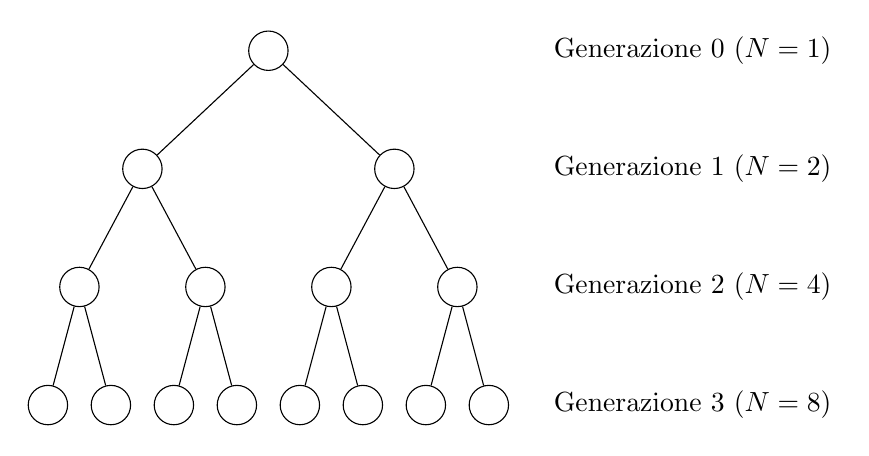
\begin{tikzpicture}[node distance=15mm, main node/.style={circle,draw,minimum size=5mm}]%
  \node at (0, 0) {};
  \node[main node] (1) {};
  \node (l1)[right of=1,xshift=2cm,anchor=west] {Generazione 0 ($N=1$)};
  
  \node[main node] (11) [below of=1, xshift=-16mm] {};
  \node[main node] (12) [below of=1, xshift=16mm] {};
  \draw[] (1) -- (11);
  \draw[] (1) -- (12);
  \node (l2) [below of=l1] {Generazione 1 ($N=2$)};

  \node[main node] (111) [below of=11, xshift=-8mm] {};
  \node[main node] (112) [below of=11, xshift=8mm] {};
  \node[main node] (121) [below of=12, xshift=-8mm] {};
  \node[main node] (122) [below of=12, xshift=8mm] {};
  \draw[] (11) -- (111);
  \draw[] (11) -- (112);
  \draw[] (12) -- (121);
  \draw[] (12) -- (122);
  \node (l3) [below of=l2] {Generazione 2 ($N=4$)};

  \node[main node] (1111) [below of=111, xshift=-4mm] {};
  \node[main node] (1112) [below of=111, xshift=4mm] {};
  \node[main node] (1121) [below of=112, xshift=-4mm] {};
  \node[main node] (1122) [below of=112, xshift=4mm] {};
  \node[main node] (1211) [below of=121, xshift=-4mm] {};
  \node[main node] (1212) [below of=121, xshift=4mm] {};
  \node[main node] (1221) [below of=122, xshift=-4mm] {};
  \node[main node] (1222) [below of=122, xshift=4mm] {};
  \draw[] (111) -- (1111);
  \draw[] (111) -- (1112);
  \draw[] (112) -- (1121);
  \draw[] (112) -- (1122);
  \draw[] (121) -- (1211);
  \draw[] (121) -- (1212);
  \draw[] (122) -- (1221);
  \draw[] (122) -- (1222);
  \node (l4) [below of=l3] {Generazione 3 ($N=8$)};
\end{tikzpicture}

}{
    \caption{Schematizzazione del nostro modello semplificato per la crescita
      di una popolazione di batteri. Sotto le nostre ipotesi il numero totale
      $N$ di batteri cresce esponenzialmente con il numero di generazioni.}
    \label{fig:popolazione_batteri}
  }
\end{figure}

Possiamo anche farci la domanda opposta, ovverosia: quante generazioni
dobbiamo attendere per arrivare ad un numero fissato $N$ di batteri? La risposta
è ovvia:
\begin{align}\label{eq:crescita_batteri_inversa}
  n = \llog[2]N.
\end{align}

\begin{examplebox}
  \begin{example}\label{exp:popolazione_batteri}
    Nel nostro modellino di popolazione batterica, assumendo un tempo di
    generazione di $t_\text{gen} = 20$~min, quanto tempo (e quante generazioni)
    dobbiamo attendere perché il numero di batteri ecceda il numero
    di protoni nell'Universo (diciamo $10^{80}$)? La risposta segue direttamente
    dalla~\eqref{eq:crescita_batteri_inversa} ed è 266, per un tempo pari
    a meno di $4$~giorni.
  \end{example}

  \begin{example}[Il foglio e la Luna]\label{exp:carta_luna}
    Quante volte dobbiamo piegare un foglio di carta per arrivare fino alla
    Luna? Lo spessore del foglio raddoppia ad ogni piegatura, per cui segue
    l'analogo della legge~\eqref{eq:crescita_batteri}. Il rapporto tra la
    distanza Terra-Luna ($\sim 380\,000$~km) e lo spessore di un foglio di carta
    ($\sim 0.1$~mm) è dell'ordine di $\sim 3.8 \times 10^{12}$, e la risposta
    cercata è 42.
  \end{example}
\end{examplebox}

Gli esempi~\ref{exp:popolazione_batteri} e \ref{exp:carta_luna} illustrano
a dovere cosa intendiamo quando diciamo che l'esponenziale cresce
"velocemente". Per completezza dobbiamo notare anche come essi siano
completamente irrealistici. Il nostro modello per la popolazione batterica non
tiene in conto che le risorse per lo sviluppo cellulare non sono infinite per
cui in realtà la popolazione stessa, dopo una fase iniziale di sviluppo
esponenziale, tenderà necessariamente ad andare in equilibrio. D'altra parte
non è operativamente possibile piegare un foglio di carta $42$~volte
(potete fare la prova---quanto dovrebbe essere l'area di base del nostro
immaginario parallelepipedo finale?). In un certo senso potremmo dire che la
crescita esponenziale è così veloce che in natura non si può sostenere
a lungo.


\subsection{Digressione: logaritmi e ricerca binaria}

Inquadriamo il problema da un punto di vista differente. Supponiamo di avere
un elenco telefonico con $N$ elementi ordinati alfabeticamente e di essere
interessati al numero di telefono di una persona specifica---quale strategia
useremmo?

Potremmo partire dall'inizio, scorrere nome per nome l'elenco e fermarci quando
arriviamo alla persona desiderata---operare, cioè, una
\emph{ricerca sequenziale}. Così facendo dovremo controllare in media
$N/2$ numeri, ed $N$ nel caso più sfavorevole (quello cioè in cui la
persona cercata è l'ultima nell'elenco).

Oppure possiamo partire da metà dell'elenco e vedere se il nome cercato
è prima o dopo nella lista: in un passo eliminiamo metà dell'elenco, e
possiamo ripetere la procedura bisecando ogni volta la parte rimanente, che in
questo modo si dimezza ad ogni passo. Non è difficile convincersi che il
processo converge in un numero di passi minore o uguale a $\llog[2] N$.
(E per $N$ grande, $\llog[2] N$ o $N$ fa un'enorme differenza.) L'algoritmo
che abbiamo appena delineato si dice \emph{ricerca binaria} ed è ottimale
per la ricerca di un elemento in una lista ordinata.

\begin{figure}[htb!]
  \autohstack{
    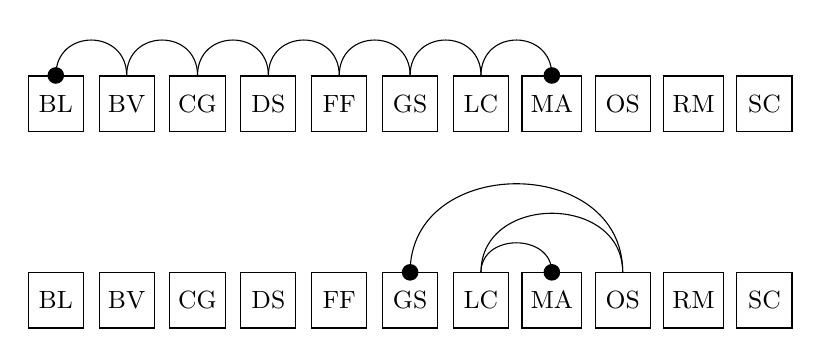
\begin{tikzpicture}[node distance=9mm, main node/.style={rectangle,draw,minimum size=7mm}]%
  \node at (0, 0) {};
  {\small
    \node[main node] (BL) {BL};
    \node[main node] (BV) [right of=BL] {BV};
    \node[main node] (CG) [right of=BV] {CG};
    \node[main node] (DS) [right of=CG] {DS};
    \node[main node] (FF) [right of=DS] {FF};
    \node[main node] (GS) [right of=FF] {GS};
    \node[main node] (LC) [right of=GS] {LC};
    \node[main node] (MA) [right of=LC] {MA};
    \node[main node] (OS) [right of=MA] {OS};
    \node[main node] (RM) [right of=OS] {RM};
    \node[main node] (SC) [right of=RM] {SC};
  }
  \draw [out=90,in=90,distance=0.6cm] (BL.north) to (BV.north);
  \draw [out=90,in=90,distance=0.6cm] (BV.north) to (CG.north);
  \draw [out=90,in=90,distance=0.6cm] (CG.north) to (DS.north);
  \draw [out=90,in=90,distance=0.6cm] (DS.north) to (FF.north);
  \draw [out=90,in=90,distance=0.6cm] (FF.north) to (GS.north);
  \draw [out=90,in=90,distance=0.6cm] (GS.north) to (LC.north);
  \draw [out=90,in=90,distance=0.6cm] (LC.north) to (MA.north);

  \fill (BL.north) circle [radius=3pt];
  \fill (MA.north) circle [radius=3pt];
  
  {\small
    \node[main node] (BL) at (0, -2.5) {BL};
    \node[main node] (BV) [right of=BL] {BV};
    \node[main node] (CG) [right of=BV] {CG};
    \node[main node] (DS) [right of=CG] {DS};
    \node[main node] (FF) [right of=DS] {FF};
    \node[main node] (GS) [right of=FF] {GS};
    \node[main node] (LC) [right of=GS] {LC};
    \node[main node] (MA) [right of=LC] {MA};
    \node[main node] (OS) [right of=MA] {OS};
    \node[main node] (RM) [right of=OS] {RM};
    \node[main node] (SC) [right of=RM] {SC};
  }

  \draw [out=90,in=90,distance=1.5cm] (GS.north) to (OS.north);
  \draw [out=90,in=90,distance=1cm] (OS.north) to (LC.north);
  \draw [out=90,in=90,distance=0.5cm] (LC.north) to (MA.north);

  \fill (GS.north) circle [radius=3pt];
  \fill (MA.north) circle [radius=3pt];
\end{tikzpicture}


  }{
    \caption{Illustrazione di due strategie di ricerca delle iniziali
      "MA" in una lista di 11 iniziali (fittizie) ordinate alfabeticamente.
      La ricerca sequenziale termina in 8 passi, quella binaria in 4 (o
      3, a seconda di come definiamo l'algoritmo di bisezione). I cerchi
      neri indicano i punti di inizio e fine della ricerca.}
    \label{fig:ricerca_binaria}
  }
\end{figure}

\begin{examplebox}
  \begin{example}
    In un elenco telefonico con $11$ persone una ricerca sequenziale richiede
    al massimo $11$ passi ed una ricerca binaria $4$. (Un esempio specifico
    è mostrato in figura~\ref{fig:ricerca_binaria}, in cui per brevità
    si è usato iniziali fittizie al posto dei nomi completi.) In questo caso
    la differenza non è impressionante, ma con un elenco di $10\,000\,000$
    di persone una ricerca sequenziale richiede al massimo $10\,000\,000$ di
    passi, mentre una ricerca binaria ne richiede al massimo
    $\llog[2]{10\,000\,000} < 24$.
  \end{example}
\end{examplebox}


\subsection{Ancora sui logaritmi: il concetto di decade}
\label{sec:decadi}

Vi è un'altra proprietà dei logaritmi che utilizzeremo sovente in seguito:
quella di trasformare prodotti in somme e quozienti in differenze. In formule:
\begin{align*}
  \ln (x_1 x_2) = \ln x_1 + \ln x_2 \quad \text{e} \quad
  \ln \left(\frac{x_1}{x_2}\right) = \ln x_1 - \ln x_2.
\end{align*}
\`E in base alla seconda di queste identità che, come vedremo tra un attimo,
si dà una definizione operativa di decade---e, in contesti diversi, ottave,
toni e semitoni.

Tecnicamente una decade è un intervallo di valori numerici i cui estremi
stiano tra loro nel rapporto di 1 a 10. Dati allora due numeri $x_1$ ed $x_2$,
la loro distanza in decadi è data da
\begin{align}\label{eq:distanza_in_decadi}
  \text{dex}(x_1, x_2) = \log\left( \frac{x_2}{x_1} \right).
\end{align}

\begin{examplebox}
  \begin{example}
    Il numero di decadi comprese tra i valori $10^n$ e $10^{n + m}$ si calcola
    banalmente come
    \begin{align*}
      \text{dex}(10^n, 10^{n + m}) = \log\left(\frac{10^{n + m}}{10^n}\right) = \log(10^m) = m.
    \end{align*}
    Ci sono cioè 3 decadi tra, e.g., $10$ e $10000$ oppure $1$ e $1000$
    e due decadi, e.g., tra $0.1$ e $10$.
  \end{example}
\end{examplebox}


\section{Una breve digressione: il suono}

Il suono è essenzialmente un'onda meccanica che si propaga in un mezzo
(ad esempio l'aria) e che noi percepiamo come una
variazione di pressione sul timpano. Come tutte le onde, è caratterizzato
dalla sua \emph{frequenza} (e dalla lunghezza d'onda, ad essa legata dalla
velocità di propagazione) e dalla sua \emph{intensità}.
Il suono è profondamente legato ai logaritmi in almeno due modi diversi, per
cui approfittiamo del bagaglio di conoscenze che abbiamo appena acquisito per
una breve digressione.


\subsection{L'altezza del suono: l'ottava}

L'\emph{altezza} è ciò che distingue un suono acuto da un suono grave,
ed è determinato essenzialmente dalla frequenza del suono in questione.
L'orecchio umano è sensibile in un intervallo di frequenze
compreso tra circa $20$~Hz e circa $20$~kHz---e questo intervallo (di tre
decadi) si dice spettro udibile. Tanto per fissare le idee: il DO più grave
del pianoforte moderno è a $32.7032$~Hz e quello più acuto a $4186.01$~Hz;
il LA dell'ottava centrale è, per definizione, a $440$~Hz e corrisponde anche
all'altezza del diapason che si usa per accordare gli strumenti.

In modo del tutto analogo alla decade, l'\emph{ottava} è un intervallo di
frequenze i cui estremi stanno tra loro nel rapporto $1:2$. Nel linguaggio dei
logaritmi, il numero di ottave tra due frequenze $\nu_1$ e $\nu_2$ è
\begin{align}\label{eq:distanza_in_ottave}
  \text{ottave}(\nu_1, \nu_2) = \llog[2]\left( \frac{\nu_2}{\nu_1} \right).
\end{align}
Nel sistema musicale occidentale l'ottava è a sua volta divisa in $12$
semitoni, di solito equispaziati logaritmicamente secondo il cosiddetto
temperamento equabile. Nella nostra notazione il numero di semitoni tra due
frequenze è dato semplicemente da
\begin{align}\label{eq:distanza_in_semitoni}
  \text{semitoni}(\nu_1, \nu_2) = 12\llog[2]\left( \frac{\nu_2}{\nu_1} \right).
\end{align}

\begin{examplebox}
  \begin{example}
    Il DO più grave e quello più acuto del pianoforte distano tra loro
    esattamente $\llog[2](4186.01/32.7032) = 7$ ottave o, equivalentemente,
    $84$~semitoni.
  \end{example}
\end{examplebox}

La~\eqref{eq:distanza_in_semitoni} può essere banalmente invertita per
trovare la costante moltiplicativa che lega due frequenze che distino tra di
loro esattamente un semitono
\begin{align}
  \frac{\nu_2}{\nu_1} = 2^{\frac{1}{12}} =\sqrt[12]{2} \approx 1.0594630943592953.
\end{align}
Il numero irrazionale $\sqrt[12]{2}$ è cioè quello che definisce il rapporto
tra le frequenze che identificano il semitono temperato. A partire da esso
(e dai $440$~Hz del LA di centro) possiamo costruire, e.g., la mappa delle
frequenze corrispondenti ai testi del pianoforte.

Incidentalmente, la frequenza fondamentale di una corda vibrante può essere
espressa in funzione della lunghezza $\ell$, della tensione $\tau$ e della
densità lineare di massa $\mu$ della corda stessa attraverso la legge di Marsenne
\begin{align}\label{eq:legge_di_marsenne}
  \nu = \frac{1}{2\ell}\sqrt{\frac{\tau}{\mu}}
\end{align}
ed è inversamente proporzionale ad $\ell$. Le tastiere degli strumenti a corda
(e.g., la chitarra) saranno dunque costruite in modo che le distanze dal
ponticello di due tasti contigui seguano una legge simile
alla~\eqref{eq:distanza_in_semitoni}
\begin{align}\label{eq:distanza_tasti}
  \frac{\ell_2}{\ell_1} = \frac{\nu_1}{\nu_2} =
  2^{-\frac{1}{12}} \approx 0.9438743126816935.
\end{align}


\subsection{Il volume sonoro}

Il volume di un suono è determinato dalla pressione $P$ che l'onda sonora esercita
sul timpano, ed il volume percepito $L_p$ è misurato in decibel (dB) rispetto ad
una pressione di riferimento $P_0$:
\begin{align}\label{eq:decibel}
  L_p = 20\log\left( \frac{P}{P_0} \right)~\text{[dB]}.
\end{align}
La pressione di riferimento viene anche detta \emph{soglia di udibilità}, ed è
convenzionalmente posta a $20~\mu$Pa. Una pressione sonora di $20~\mu$Pa
corrisponde ad un livello di $0$~dB, che è, appunto, il volume sonoro più basso
che l'orecchio umano è in grado di percepire in aria.

Come è possibile che il nostro orecchio sia sensibile ad una pressione di $20~\mu$Pa
quando la pressione atmosferica media è di $101\,325$~Pa---cioè più grande di quasi
10~ordini di grandezza?
Il punto fondamentale è che la $P$ nella~\eqref{eq:decibel} si riferisce alla
componente \emph{variabile nel tempo} della pressione---e, più precisamente,
al suo scarto quadratico medio, ma per questo dovremo aspettare ancora un po'.
La pressione atmosferica è approssimativamente costante nel tempo, almeno sui
tempi scala delle frequenze acustiche, ed è applicata su entrambe le facce
della membrana del timpano; le variazioni di pressione sono quelle che fanno
vibrare la membrana stessa e ci danno la percezione del suono. (Detto questo,
la sensibilità dell'orecchio umano rimane niente meno che impressionante.
In termini circuitali l'orecchio è un condensatore perfetto che filtra la
componente continua della pressione.)

\begin{figure}[htb!]
  \autohstack{
    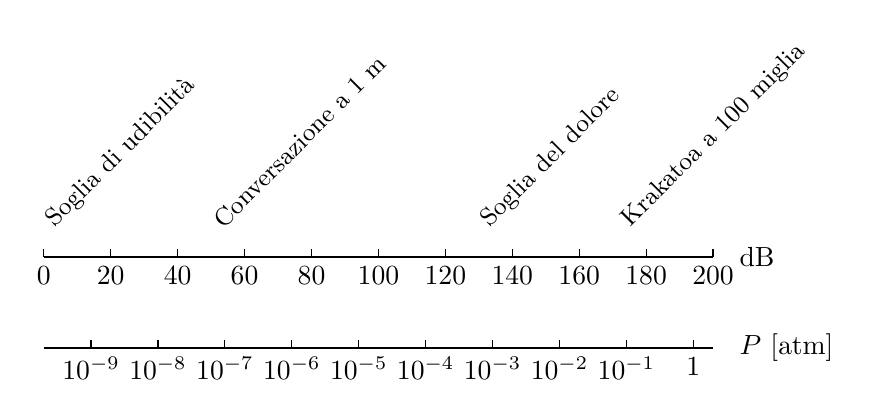
\begin{tikzpicture}[declare function={dbdist(\x)=\xscale*20*(10+\x-log10(1.97));}]%
  \node at (0, 0) {};
  \pgfmathsetmacro{\xscale}{0.0425}

  \pgfmathsetmacro{\y}{0.25}
  {\small
    \node[anchor=west,rotate=45] at (\xscale*0, \y) {Soglia di udibilit\`a};
    \node[anchor=west,rotate=45] at (\xscale*50, \y) {Conversazione a $1$~m};
    \node[anchor=west,rotate=45] at (\xscale*130, \y) {Soglia del dolore};
    \node[anchor=west,rotate=45] at (\xscale*172, \y) {Krakatoa a~100 miglia};
  }

  \pgfmathsetmacro{\y}{-0.1}
  \draw[thick] (0,\y) -- (\xscale*200,\y);
  \node[anchor=west] at (\xscale*205,\y) {dB};
  \foreach \x in {0.,20,...,200}
  \draw (\x*\xscale,\y+0.1) -- (\x*\xscale,\y) node[anchor=north]
        {$\pgfmathprintnumber{\x}$};

  \pgfmathsetmacro{\y}{-1.25}
  \draw[thick] (0,\y) -- (\xscale*200,\y);
  \node[anchor=west] at (\xscale*205,\y) {$P$~[atm]};
  \draw ({dbdist(-9)},\y+0.1) -- ({dbdist(-9)},\y) node[anchor=north] {$10^{-9}$};
  \draw ({dbdist(-8)},\y+0.1) -- ({dbdist(-8)},\y) node[anchor=north] {$10^{-8}$};
  \draw ({dbdist(-7)},\y+0.1) -- ({dbdist(-7)},\y) node[anchor=north] {$10^{-7}$};
  \draw ({dbdist(-6)},\y+0.1) -- ({dbdist(-6)},\y) node[anchor=north] {$10^{-6}$};
  \draw ({dbdist(-5)},\y+0.1) -- ({dbdist(-5)},\y) node[anchor=north] {$10^{-5}$};
  \draw ({dbdist(-4)},\y+0.1) -- ({dbdist(-4)},\y) node[anchor=north] {$10^{-4}$};
  \draw ({dbdist(-3)},\y+0.1) -- ({dbdist(-3)},\y) node[anchor=north] {$10^{-3}$};
  \draw ({dbdist(-2)},\y+0.1) -- ({dbdist(-2)},\y) node[anchor=north] {$10^{-2}$};
  \draw ({dbdist(-1)},\y+0.1) -- ({dbdist(-1)},\y) node[anchor=north] {$10^{-1}$};
  \draw ({dbdist(0)},\y+0.1) -- ({dbdist(0)},\y) node[anchor=north] {$1$};
\end{tikzpicture}

  }{
    \caption{Illustrazione della scala dei decibel e relazione con la pressione
      atmosferica. La soglia di udibilità ($20~\mu$Pa) corrisponde ad una
      variazione di pressione nel tempo di circa $2 \times 10^{-10}$~atm, una
      normale conversazione ($40$--$60$~dB) si attesta a $\sim 10^{-7}$~atm e la
      soglia del dolore ($130$~dB) è a circa $10^{-3}$~atm.}
    \label{fig:decibel}
  }
\end{figure}

Torniamo alla~\eqref{eq:decibel}. La scelta di questa unità di misura curiosa,
il decibel, riflette il fatto che la nostra percezione del suono non scala
in modo lineare ma, semmai, logaritmico con la pressione sonora, come
illustrato in figura~\ref{fig:decibel}. (Il nostro orecchio è in grado di
percepire la differenza di $100~\mu$Pa fra $100~\mu$Pa e $200~\mu$Pa, ma la
stessa differenza tra $10.0$ e $10.1$~mPa risulta del tutto impercettibile.)
Così, a fronte di una soglia di udibilità di $20~\mu$Pa
($\sim 2\times10^{-10}$~atm), una normale conversazione tra due persone ad
$1$~m di distanza corrisponde ad una pressione sonora di $40$--$60$~dB
($\sim 10^{-7}$~atm) e la soglia del dolore è convenzionalmente
fissata a $130$~dB, che è ancora più piccolo di un millesimo di~atm.
Vedremo nella sezione~\ref{sec:non_lin_scales} che la scala logaritmica è
quella più appropriata per rappresentare grandezze di questo tipo, ed in
effetti la figura~\ref{fig:decibel} ne è un primo esempio.

Vista in termini della pressione (statica) atmosferica, la variazione di
pressione corrispondente ad un qualsiasi fenomeno che classifichiamo come
\emph{suono} su scala umana è piccola. Se facessimo il grafico corrispondente
della pressione sul timpano in funzione del tempo, sarebbe un grafico
noioso---virtualmente indistinguibile da una linea orizzontale a $\sim 100$~kPa,
a meno di non sopprimere gli zeri.
Udito distintamente fino a $3000$~km di distanza, e con un livello sonoro
stimato di $172$~dB a $100$~km, l'esplosione del vulcano dell'isola di Krakatoa
(avvenuta il 27 agosto 1883) è considerato il suono più intenso (in aria)
registrato sulla Terra nella storia moderna. Ma persino $172$~dB corrispondono
ad una variazione di pressione di meno del $10\%$ della pressione atmosferica.
(Per completezza, i KISS detengono il record di livello sonoro ad un concerto
rock---un misero $136$~dB misurato ad Ottawa nel 2009.\footnote{\url{https://en.wikipedia.org/wiki/Loudest_band_in_the_world}})
$194$~dB è il limite fisico oltre il quale la componente variabile della
pressione è uguale alla pressione atmosferica, ed un'onda sonora non può propagarsi
in aria senza distorsioni.


\section{Scale non lineari}
\label{sec:non_lin_scales}

Riprendiamo il filo del nostro discorso. Per l'occhio umano è relativamente
semplice percepire deviazioni da un andamento lineare. Non è così semplice,
di contrasto, distinguere immediatamente i grafici cartesiani di funzioni i cui
andamenti siano qualitativamente simili---ad esempio $x^2$ e $x^4$.

\begin{table}[!htb]
  \tablehstack{
    \centering\begin{tabular}{lll}
        \hline
        Pianeta & $a$~[U.A.] & $T$~[anni] \\
        \hline
        \hline
        Mercurio & $0.3870993$ & $0.2408467$  \\
        Venere   & $0.723336$  & $0.61519726$ \\
        Terra    & $1.000003$  & $1.0000174$  \\
        Marte    & $1.52371$   & $1.8808158$  \\
        Giove    & $5.2029$    & $11.862615$  \\
        Saturno  & $9.537$     & $29.447498$  \\
        Urano    & $19.189$    & $84.016846$  \\
        Nettuno  & $30.0699$   & $164.79132$  \\
        \hline
      \end{tabular}
  }{
    \caption{Parametri orbitali (semiasse maggiore dell'orbita $a$ e periodo di
      rivoluzione $T$) dei pianeti del Sistema Solare, da
      \url{http://www.princeton.edu/~willman/planetary_systems/Sol/}.
      (Per completezza $1~\text{U.A.} = 149\,597\,870\,700$~m e
      $1~\text{anno Giuliano} = 365.25$~giorni).
      Assumeremo per semplicità che tutte le cifre siano significative, anche se
      non è banale associare incertezze ai dati, poiché i parametri
      orbitali sono soggetti a complicate variazioni secolari.}
    \label{tab:sistema_solare}
  }
\end{table}

A titolo illustrativo, la tabella~\ref{tab:sistema_solare} contiene alcuni dati
orbitali (semiasse maggiore dell'orbita $a$ e periodo di rivoluzione $T$) degli
8 pianeti del Sistema Solare (Plutone escluso). Un grafico $xy$ dei dati nella
tabella, come quello in figura~\ref{fig:sistema_solare_lin}, suggerisce che le
due quantità siano legate tra di loro da una qualche relazione funzionale---ma
chiaramente questa relazione non è di tipo lineare, per cui, arrivati a
questo punto, non sapremmo bene come procedere, dato il nostro bagaglio di
conoscenze. Quale tipo di legge potrebbe legare il periodo dell'orbita al
semiasse?
(Un ulteriore problema, per certi versi secondario, risiede nel fatto che i
nostri dati variano su diversi ordini di grandezza, per cui nel grafico i 4
pianeti più vicini al sole tendono ad essere schiacciati sull'origine
degli assi. Ci torneremo in seguito.)

\pgffigone{sistema_solare_lin}{
  Grafico $xy$ dei parametri orbitali (semiasse maggiore dell'orbita e periodo
  di rivoluzione) degli 8 pianeti del Sistema Solare, come mostrati nella
  tabella~\ref{tab:sistema_solare}. Per la terza legge di
  Keplero~\eqref{eq:legge_di_keplero}, che abbiamo derivato per via dimensionale
  nell'esempio~\ref{exp:calcolo_dimensionale_keplero}, ci aspettiamo che
  i punti si dispongano su una legge di potenza con esponente $3/2$, ma ovviamente
  la cosa non è banale da verificare quantitativamente guardando la figura.
  Notiamo esplicitamente che, in questa rappresentazione, i 4 pianeti più vicini
  al sole tendono ad essere schiacciati sull'origine e non sono facilmente
  distinguibili.
}

In alcune situazioni funzioni complesse possono essere \emph{linearizzate}
mediante opportuni cambiamenti di variabili. \`E possibile in tal modo
evidenziare caratteristiche che altrimenti sarebbero estremamente difficili da
cogliere dalla semplice rappresentazione grafica. In questa sezione ci
occuperemo di due classi di funzioni estremamente utili in Fisica---le leggi di
potenza e gli esponenziali. Vedremo che in entrambi i casi si può linearizzare
il problema usando scale logaritmiche.


\subsection{Di nuovo sulle decadi: la scala logaritmica}

Come abbiamo visto nel caso del suono, in natura esistono fenomeni che scalano
in modo intrinsecamente logaritmico. La definizione di decade~\eqref{eq:distanza_in_decadi}
che abbiamo dato nella sezione~\ref{sec:decadi} è importante perché ci permette di costruire
scale graduate non lineari in cui la distanza (misurata in~cm) tra due punti sia
proporzionale alla distanza in decadi tra i valori corrispondenti, come illustrato
in figura~\ref{fig:costruzione_asse_logaritmico}.
Una scala di questo tipo si dice \emph{scala logaritmica}, ed è spesso conveniente
per rappresentare fenomeni non lineari.

\begin{figure}[htb!]
  \autohstack{
    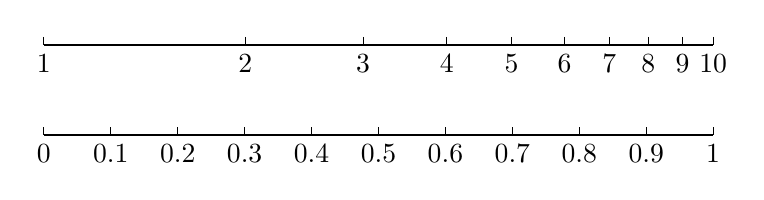
\begin{tikzpicture}[declare function={logdist(\x)=\xscale*log10(\x);}]%
  \node at (0, 0) {};
  \pgfmathsetmacro{\xscale}{8.5}
  \pgfmathsetmacro{\y}{-1.25}
  \draw[thick] (0,\y) -- (\xscale,\y);
  \foreach \x in {0.,0.1,...,1.1}
  \draw (\x*\xscale,\y+0.1) -- (\x*\xscale,\y) node[anchor=north]
        {$\pgfmathprintnumber{\x}$};
        
  \pgfmathsetmacro{\y}{-0.1}
  \draw[thick] (0,\y) -- (\xscale,\y);
  \foreach \x in {1,...,10}
  \draw ({logdist(\x)},\y+0.1) -- ({logdist(\x)},\y) node[anchor=north]
        {$\pgfmathprintnumber{\x}$};
\end{tikzpicture}

  }{
    \caption{Costruzione di un asse in scala logaritmica. Assumendo una
      lunghezza unitaria per la decade, la distanza tra. e.g.,  $1$ e $2$
      è pari a $\log(2/1) \approx 0.301$.}
    \label{fig:costruzione_asse_logaritmico}
  }
\end{figure}

Così in scala logaritmica la distanza fisica tra $1$ e $10$ è identica a
quella tra $10$ e $100$ o $0.01$ e $0.1$. Va da sé che lo $0$ non può
essere rappresentato su scala logaritmica in quanto la distanza da esso
di un qualsiasi valore positivo divergerebbe---che è sostanzialmente una
conseguenza del fatto che
\begin{align*}
  \lim_{x\rightarrow 0^+} \log(x) = -\infty.
\end{align*}


\subsection{Leggi di potenza e grafici bilogaritmici}
\label{subsec:bilog}

Si dice \emph{legge di potenza} una funzione di una variabile reale $x$,
la cui espressione analitica sia della forma
\begin{align}\label{eq:legge_di_potenza}
  y(x; C, \Gamma) = Cx^\Gamma.
\end{align}
I parametri $C$ e $\Gamma$ si dicono rispettivamente costante ed esponente della
legge di potenza; a seconda del contesto $\Gamma$ viene detto talvolta anche
indice spettrale o semplicemente indice. In Fisica gli esempi di legge di potenza
sono innumerevoli, come illustrato negli
esempi~\ref{exp:pl_moto_accelerato}--\ref{exp:pl_raggi_cosmici}.

\begin{examplebox}
  \begin{example}\label{exp:pl_moto_accelerato}
    La legge spazio tempo per un corpo in caduta libera sotto l'azione della gravità
    terrestre (con le opportune condizioni iniziali, ovvero nella forma
    $s(t) = \nicefrac{1}{2}gt^2$) è una legge di potenza con $C = \nicefrac{g}/{2}$
    ed esponente $\Gamma = 2$.
  \end{example}

  \begin{example}
    La relazione tra il periodo e la lunghezza di un pendolo in
    approssimazione di piccole oscillazioni è una legge di potenza con
    $C = \nicefrac{2\pi}{\sqrt{g}}$ e $\Gamma = \nicefrac{1}{2}$.
  \end{example}

  \begin{example}
    Una retta passante per l'origine $y(x) = Cx$ è una legge di potenza con
    esponente $\Gamma = 1$.
  \end{example}

  \begin{example}
    La terza legge di Keplero~\eqref{eq:legge_di_keplero} è una legge di
    potenza con esponente $\Gamma = \nicefrac{3}{2}$.
  \end{example}

  \begin{example}
    Il reddito pro-capite annuo è (approssimativamente) descritto da una
    distribuzione di probabilità a legge di potenza. (Come osservato da
    Pareto alla fine del XIX secolo, la maggior parte della ricchezza è
    posseduto da un piccolo numero di persone.)
  \end{example}

  \begin{example}\label{exp:pl_raggi_cosmici}
    Lo spettro in energia dei raggi cosmici può essere ragionevolmente
    descritto da una legge di potenza con indice $\Gamma \approx -2.75$ su quasi
    dieci ordini di grandezza in energia (si tratta di uno degli esempi più
    spettacolari in natura).
  \end{example}
\end{examplebox}

Calcolando il logaritmo in base $10$ di entrambi i membri della~\eqref{eq:legge_di_potenza},
ovverosia operando il cambio di variabile
\begin{align*}
  \begin{cases}
    x' = \log(x)\\
    y' = \log(y)
  \end{cases}
\end{align*}
essa può essere convenientemente riscritta come:
\begin{align}\label{eq:legge_di_potenza_newvar}
  y' = \log(y) = \log(Cx^\Gamma) = \log(C) + \Gamma\log(x) = \log(C) + \Gamma x'.
\end{align}
Nelle nuove variabili la ~\eqref{eq:legge_di_potenza} è una retta il cui
coefficiente angolare coincide con l'esponente della legge di potenza iniziale.
Questo ci suggerisce che, data una serie di punti sperimentali $(x_i, y_i)$, un
grafico dei valori di $\log(y_i)$ in funzione di $\log(x_i)$ sia un modo
immediato per verificare se i dati sono legati tra di loro da una relazione
funzionale di tipo legge di potenza. In realtà, in pratica, si preferisce
usare grafici con assi in scala logaritmica, come mostrato in
figura~\ref{fig:costruzione_asse_logaritmico}.

Un grafico in cui sia l'asse delle $x$ che quello delle $y$ sono in scala
logaritmica si dice \emph{grafico bilogaritmico}. Un foglio di carta
prestampato con una coppia di assi ortogonali graduati in scala logaritmica
(tipicamente corredati di griglie) si dice \emph{carta bilogaritmica}.
La carta bilogaritmica offre due ovvi vantaggi. Il primo è che in fase di
creazione del grafico non è necessario calcolare i logaritmi dei valori
sperimentali: è sufficiente usare gli assi graduati per mettere i punti sul
grafico (questo in effetti non fa necessariamente una grande differenza se si
utilizza un programma al calcolatore per realizzare il grafico).
Il secondo, più importante, è che in fase di lettura del grafico
è immediato ricavare i valori delle grandezze fisiche che i punti
rappresentano---senza bisogno di elevamenti a potenza per invertire la
trasformazione iniziale.

\pgffigone{sistema_solare_log}{
  Grafico $xy$ in scala bilogaritmica dei parametri orbitali (semiasse maggiore
  dell'orbita e periodo di rivoluzione) degli 8 pianeti del Sistema Solare,
  come mostrati nella tabella~\ref{tab:sistema_solare} e nella
  figura~\ref{fig:sistema_solare_lin} (su scala lineare).
  In questa rappresentazione i punti si dispongono su di una retta, il che
  indica che le due grandezze sono legate tra di loro da una relazione
  funzionale di tipo legge di potenza, in accordo con
  la~\eqref{eq:legge_di_keplero}. \`E evidente, inoltre, che risulta molto
  più semplice distinguere tra loro i pianeti più piccoli rispetto alla
  rappresentazione originale in scala lineare.
}

Torniamo allora al nostro esempio dei dati orbitali relativi ai pianeti del
Sistema Solare, che abbiamo già illustrato nella
tabella~\ref{tab:sistema_solare} e nella figura~\ref{fig:sistema_solare_lin}.
Il grafico corrispondente in scala bilogaritmica è mostrato in
figura~\ref{fig:sistema_solare_log}, da cui è evidente che i punti si
dispongono su di una retta. Questo ci permette di concludere che il legame
funzionale tra il periodo di rivoluzione ed il semiasse maggiore dell'orbita
è del tipo legge di potenza, come ci aspettavamo dalla terza legge di
Keplero (cosa che non era affatto ovvio né dalla rappresentazione in forma
tabellare, né dal grafico di dispersione in scala lineare).

I grafici in carta bilogaritmica permettono di stimare \emph{visivamente} i
parametri della legge di potenza che meglio descrive i dati. Presi due punti sulla
retta di \fit, il coefficiente angolare si ricava dalla~\eqref{eq:legge_di_potenza_newvar}
come
\begin{align}\label{eq:legge_di_potenza_fit_index}
  \Gamma = \frac{y'_2 - y'_1}{x'_2 - x'_1} =
  \frac{\log(y_2) - \log(y_1)}{\log(x_2) - \log(x_1)} =
  \frac{\log(y_2/y_1)}{\log(x_2/x_1)} =
  \frac{\text{dex}(y_1, y_2)}{\text{dex}(x_1, x_2)}.
\end{align}
\emph{L'esponente della legge di potenza è dunque una misura di quante decadi ci
spostiamo sull'asse delle $y$ quando ci spostiamo di una decade sull'asse delle
$x$.} Nel caso della figura~\ref{fig:sistema_solare_log} vediamo che dal punto
corrispondente alla Terra all'angolo in alto a destra del grafico ci spostiamo
di circa 2 decadi sulla $x$ e circa 3 decadi sulla $y$---ergo, l'indice della
legge di potenza è $\Gamma \approx \nicefrac{3}{2}$, come atteso
Se poi, nella~\eqref{eq:legge_di_potenza_newvar}, poniamo $x' = 0$, si ha
$y' = \log(C)$, ovvero $y = C$. Ma la condizione $x' = 0$ corrisponde, nelle
variabili non trasformate, a $x = 1$, per cui \emph{in scala bilogaritmica
l'intercetta non è l'intercetta con l'asse $x = 0$ (che per altro non esiste),
ma l'intercetta con l'asse $x = 1$.}


\subsection{Un'applicazione grafica interessante: l'inarmonicità del pendolo
  in scala bilogaritmica}

Nella sezione~\ref{sec:piccole_oscillazioni} abbiamo discusso in dettaglio il
significato dell'approssimazione di piccole oscillazioni nel caso del pendolo
semplice, e derivato la condizione esplicita~\eqref{eq:condizione_piccole_oscillazioni}
entro la quale una data ampiezza di oscillazione $\theta_0$ può essere considerata
piccola.
La figura~\ref{fig:piccole_oscillazioni} è utile perché dà un'idea immediata
della deviazione del periodo dal limite di piccole oscillazioni in funzione di $\theta_0$.
Da un punto di vista quantitativo è però estremamente difficile ricavarne
informazioni numeriche per $\theta_0 \leq 10^\circ$, poiché la curva è
graficamente indistinguibile dalla retta orizzontale $T/T_0 = 1$. Possiamo
dire che per $\theta_0 \leq 10^\circ$ la deviazione del periodo dal valore
asintotico è minore dell'$1\%$, ma non molto di più.

In situazioni come questa un uso \emph{creativo} delle scale logaritmiche
permette spesso di rappresentare graficamente l'informazione in un modo
più immediato ed efficace. Se vogliamo dare enfasi all'inarmonicità per
angoli piccoli, la prima cosa da fare è sottrarre il valore costante
$T/T_0 = 1$ che non influisce sulla forma della curva. Metteremo sul grafico,
cioè, la quantità
\begin{align}
  \delta(\theta_0) = \frac{T(\theta_0)}{T_0} - 1 = \frac{T(\theta_0) - T_0}{T_0}.
\end{align}
$\delta(\theta_0)$ rappresenta la \emph{deviazione relativa} del periodo del
pendolo dal valore asintotico per piccole oscillazioni. Il grafico in scala
bilogaritmica è mostrato in~figura~\ref{fig:piccole_oscillazioni_log}.

\pgffigone{piccole_oscillazioni_log}{
  Deviazione dall'armonicità del pendolo semplice in funzione dell'ampiezza
  di oscillazione $\theta_0$. La grandezza rappresentata sull'asse delle
  ordinate si può confrontare direttamente con l'errore relativo sulla
  misura del periodo per verificare il valore dell'ampiezza al di sotto del
  quale l'approssimazione di piccole oscillazioni può essere utilizzata.
  Notiamo esplicitamente che l'aggiunta delle griglie nel grafico facilita
  l'operazione.
}

Dobbiamo stupirci che, in questa rappresentazione, $\delta(\theta_0)$ abbia tutta
l'aria di una retta? La risposta è no, perché dalla~\eqref{eq:periodo_pendolo_theta}
segue che la nostra quantità può essere sviluppata in serie come
\begin{align*}
  \delta(\theta_0) = \frac{1}{16}\theta_0^2 +
  \frac{11}{3072}\theta_0^4 + \frac{173}{737\,280}\theta_0^6 +
  \frac{22\,931}{1\,321\,205\,760}\theta_0^8 +
  \cdots
\end{align*}
e siccome abbiamo visto che il primo termine (in $\theta_0^2$) è quello
dominante, allora $\delta(\theta_0)$ è \emph{quasi} una legge di potenza
(con indice $\Gamma \approx 2$). Ma la cosa più interessante è che la nostra
condizione di validità per l'approssimazione di piccole
oscillazioni~\eqref{eq:condizione_piccole_oscillazioni}, che possiamo
convenientemente riscrivere come
\begin{align*}
  \delta(\theta_0) \ll \frac{\sigma_T}{T_0},
\end{align*}
si legge direttamente sul grafico: dato l'errore relativo $\sigma_T/T_0$ sulla
misura del periodo è sufficiente tracciare la retta orizzontale di
equazione a $\delta(\theta_0) = \sigma_T/T_0$ e trovare l'angolo in
corrispondenza del quale questa retta interseca la funzione $\delta(\theta_0)$.
Così se misuriamo il periodo all'$1\%$ dalla figura vediamo che possiamo
utilizzare l'approssimazione di piccole oscillazioni per
$\theta_0 \ll 20$--$30^\circ$, ma se l'errore relativo è, e.g., $10^{-4}$,
allora la nostra ampiezza deve essere $\theta_0 \ll 2$--$3^\circ$.


\subsection{Funzioni esponenziali e grafici semilogaritmici}
\label{subsec:semilog}

Si dice \emph{esponenziale} una funzione di una variabile reale dipendente da
due parametri della forma
\begin{align}\label{eq:esponenziale}
  y(x; C, \lambda) = Ce^{-\lambda x},
\end{align}
in cui $C$ prende il nome di costante di normalizzazione e $\lambda$ si dice
semplicemente parametro. (In Fisica gli esponenziali sono per lo più decrescenti,
da cui il segno $-$ davanti a $\lambda$.)

\begin{examplebox}
  \begin{example}\label{exp:legge_di_newton}
    Si immerge un termometro in un misto di acqua e ghiaccio---per definizione a
    $0^\circ$. Assumendo la capacità termica del termometro trascurabile
    (cioè assumendo di avere abbastanza acqua e ghiaccio), ci aspettiamo che
    la temperatura $T$ di quest'ultimo, per la legge del raffreddamento di
    Newton, si porti esponenzialmente nel tempo dalla sua temperatura iniziale
    $T_0$ a quella ($0^\circ$) del bagno termico
    \begin{align*}
      T(t) = T_0 e^{-\lambda t}.
    \end{align*}
  \end{example}

  \begin{example}
    In un campione radioattivo il numero medio di nuclei che non sono ancora decaduti
    decade esponenzialmente nel tempo.
  \end{example}
\end{examplebox}

Nel caso, tipico, in cui la variabile indipendente rappresenti un tempo, il parametro
$\lambda$ prende il nome di tempo caratteristico o costante di decadimento; il suo
reciproco $\tau = \nicefrac{1}{\lambda}$ si dice vita media e si interpreta come
l'intervallo di tempo dopo il quale il valore della funzione si è ridotto ad un fattore
\begin{align}\label{eq:exp_decay_mean_lifetime}
  \frac{y(\tau)}{y(0)} = \frac{Ce^{-\lambda \tau}}{C} =
  \frac{Ce^{-\lambda/\lambda}}{C} = \frac{1}{e}
\end{align}
rispetto al valore iniziale. In questo caso una grandezza correlata alla vita media è il
tempo di dimezzamento, definito come il tempo dopo il quale l'ampiezza si è ridotta
ad $\nicefrac{1}{2}$ del valore iniziale, che si dimostra banalmente essere
\begin{align}\label{eq:exp_decay_half_life}
  T_{1/2} = \tau\ln2.
\end{align}

Esattamente come nel caso delle leggi di potenza, gli esponenziali si possono
linearizzare attraverso un opportuno cambio di variabili: come per le leggi di
potenza, calcoliamo il logaritmo in base dieci di entrambi i membri
della~\eqref{eq:esponenziale}:
\begin{align*}
  \log(y) = \log(Ce^{\lambda x}) = \log(C) + \lambda x\log(e).
\end{align*}
Con il cambiamento di variabile
\begin{align*}
  \begin{cases}
    x' = x \log(e)\\
    y' = \log(y)
  \end{cases}
\end{align*}
la~\eqref{eq:esponenziale} diviene
\begin{align}
  y' = \log(C) + \lambda x',
\end{align}
che è (di nuovo) l'equazione di una retta. A questo punto non stupirà il fatto
che esistono grafici \emph{semilogaritmici} e carte prestampate semilogaritmiche---e
gli esponenziali hanno la caratteristica di trasformarsi in rette in scala semilogaritmica,
come illustrato in figura~\ref{fig:temperatura_newton_lin_temperatura_newton_log}.
Osservatela attentamente, perché la cosa è istruttiva.

\pgffigtwo[hb!]{temperatura_newton_lin}{temperatura_newton_log}{
  Temperatura registrata da un termistore, di capacità termica trascurabile ed
  inizialmente a temperatura ambiente, immerso in un bagno termico a $0^\circ$C
  all'istante $t=0$ (vedi esempio~\ref{exp:legge_di_newton}).}

In scala lineare non è ovvio riconoscere un esponenziale---inoltre è difficile
leggere dal grafico i valori di temperatura per tempi grandi, che tendono ad essere
schiacciati nella parte inferiore del grafico. Nel grafico in scala semilogaritmica,
viceversa, è immediato vedere che il decadimento delle temperatura è approssimativamente
esponenziale, e si vede anche chiaramente una deviazione dall'andamento rettilineo,
che indica che il nostro modello non è perfetto. Cosa ancora più importante,
i grafici in scala semilogaritmica permettono di stimare facilmente i parametri
della funzione esponenziale che meglio descrive i dati.
Il coefficiente angolare si ricava dalla~\eqref{eq:esponenziale} come
\begin{align}\label{eq:fit_grafico_semilog}
  \lambda = \frac{y'_2 - y'_1}{x'_2 - x'_1} =
  \frac{\log(y_2) - \log(y_1)}{(x_2 - x_1)\log(e)} =
  \frac{\log(y_2/y_1)}{(x_2 - x_1)\log(e)} =
  \frac{\text{dex}(y_1, y_2)}{(x_2 - x_1)\log(e)}
\end{align}
e l'intercetta è questa volta l'intercetta con l'asse $x = 0$.

Notiamo esplicitamente che un metodo alternativo per stimare graficamente $\lambda$
è quello di utilizzare la~\eqref{eq:exp_decay_half_life}: si traccia la retta
orizzontale con ordinata pari ad $\nicefrac{1}{2}$ del valore iniziale ed il valore
delle ascisse per cui essa intercetta con la retta di \bestfit\ corrisponde al
tempo di dimezzamento.


\section{Invarianza di scala e legge di Benford}
\label{sec:legge_di_benford}

Il modulo~\scipymodule{constants} mette a disposizione una lista estensiva
di costanti fisiche---nella versione 1.4.1 di~\scipy\ sono 442 valori che spaziano
su 115~ordini di grandezza, dai $6.2353799905 \times 10^{-65}$~C$^4$~m$^4$~J$^{-3}$
dell'unità atomica della seconda iper-polarizzabilità ai $1.356392489 \times 10^{50}$~Hz
della relazione kilogrammo-hertz. Utilizzeremo questa lista per capire se c'è
qualcosa di interessante da imparare dalla distribuzione delle occorrenze della
prima cifra (la più significativa) dei valori numerici delle costanti nel
Sistema Internazionale---mostrata in un grafico a barre nella figura~\ref{fig:legge_di_benford}.

\pgffigone{legge_di_benford}{
  Distribuzione delle occorrenze della prima cifra decimale dei valori numerici
  delle 442 costanti fisiche incluse nel modulo~\scipymodule{constants}.
  Per chiarezza, i numeri in corrispondenza delle barre indicano i valori assoluti
  delle occorrenze e le frequenze relative corrispondenti. La linea tratteggiata
  rappresenta i valori attesi secondo la legge di~Benford~\ref{eq:legge_di_benford}.
}

Prima ancora di chiederci il motivo per cui dovremmo essere interessati ad una metrica
apparentemente così bizzarra, vi è una cosa ovvia che possiamo notare dal grafico:
vi sono comparativamente molti più valori che iniziano con cifre piccole (e.g., $1$~e $2$)
di quanto non siano quelli che cominciano con cifre grandi (e.g., $8$~e $9$).
Non si tratta di un fatto estremamente contro-intuitivo? In un insieme di valori
assemblato in modo casuale non dovremmo aspettarci che la distribuzione di
probabilità della prima cifra dovrebbe essere piatta---cioè che
i numeri da $1$ a $9$ dovrebbero essere approssimativamente equiprobabili?

L'osservazione di questa apparente anomalia, oggi nota come legge di Benford, è stata
pubblicata per la prima volta nel 1881 da Simon Newcomb~\cite{newcomb}, sulla base
del fatto curioso che le prime pagine delle tavole dei logaritmi tendevano ad
essere molto più consumate delle ultime, e poi riscoperta ed elaborata ulteriormente
da Frank Benford nel 1938~\cite{benford}. Nel nostro linguaggio, saremmo tentati
di dire che, quando una lista di valori tende ad essere distribuita su diversi
ordini di grandezza, il modo più naturale di rappresentarla è utilizzando una
scala logaritmica come quella mostrata in figura~\ref{fig:costruzione_asse_logaritmico}.
Ma se generiamo numeri distribuiti casualmente su una scala logaritmica, quelli
che iniziano con un~1 saranno comparativamente più frequenti di quelli che iniziano
con un~2, perché la distanza fisica tra 1 e 2 è maggiore di quella tra 2 e 3, e
così via. Di più: possiamo essere quantitativi e dire che, in queste ipotesi, la
frequenza relativa attesa della cifra~$n$ sarà pari alla distanza in decadi
tra $n$ ed $n + 1$:
\begin{align}\label{eq:legge_di_benford}
  F(n) = \text{dex}(n, n + 1) = \log \left(\frac{n + 1}{n}\right) =
  \log \left(1 + \frac{1}{n}\right).
\end{align}

La linea tratteggiata in figura~\ref{fig:legge_di_benford} rappresenta proprio
le frequenze relative attese dalla~\ref{eq:legge_di_benford} e, almeno a livello
qualitativo, il livello di accordo è niente meno che sorprendente.


\summary

\begin{itemize}
\item Tabelle e grafici sono fondamentali per ordinare e rendere comprensibili
  i vostri dati e devono essere il più possibile chiari ed auto-esplicativi.
\item Dare sempre nomi chiari alle colonne delle tabelle ed
  agli assi dei grafici, ed indicate sempre le unità di misura.
\item Le incertezze devono essere mostrate in modo chiaro ed esplicito; quando
  possibile, scegliete le scale degli assi in modo che le incertezze siano ben visibili.
\item \`E bene riportare le divisioni, regolari, degli assi dei grafici,
  in modo da poter leggere le coordinate di un qualunque punto in modo
  immediato. Non è necessario che gli assi partano sempre da zero.
\item Siate creativi e annotate i grafico con le informazioni che possono essere utili.
\item La scelta dei \foreign{bin} in un istogramma è sempre arbitraria, e
  bisogna cercare il giusto compromesso.
\item Il Fisico è capace di osservare e pensare in modo \emph{logaritmico}:
  la padronanza delle scale logaritmiche è di fondamentale importanza e deve
  essere acquisita il prima possibile. Siete in grado di stimare ad occhio l'indice
  di una legge di potenza a partire da un grafico?
\end{itemize}
